\documentclass[a4paper, 12pt,twoside]{article}
\usepackage[utf8]{inputenc}
\usepackage[frenchb,noconfigs]{babel}

\usepackage{lmodern,textcomp,ifthen,graphicx,enumitem,amsmath,amsfonts,booktabs}
\numberwithin{equation}{subsection}
\usepackage[font=small,labelfont=bf]{caption}
\usepackage{csvsimple}
\renewcommand{\thefigure}{\arabic{section}.\arabic{figure}}
\renewcommand{\thetable}{\arabic{section}.\arabic{table}}

\usepackage[notes,
            titlepage,
            a4paper,
            pagenumber,
            sectionmark,
            twoside,
            fancysections]{polytechnique}
\usepackage[colorlinks=true,
            linkcolor=black,%bleu303,
            filecolor=red,
            urlcolor=bleu303,
            bookmarks=true,
            bookmarksopen=true]{hyperref}
			
%%%%%%%%%%%%%%
%% COMANDOS %%
%%%%%%%%%%%%%%


%% Importar codigo Python: \code{blah blah blah}
\newcommand{\code}[2]{
  \hrulefill
  \subsection*{#1}
  \lstinputlisting{#2}
  \vspace{2em}
}
%% Tamaño figuras
\newlength{\mylength}
\setlength{\mylength}{0.47\textwidth}

%%%%%%%%%%%%%%%%%%
%% FIN COMANDOS %%
%%%%%%%%%%%%%%%%%%

\title{Projet Simulation Numérique Aléatoire}
\subtitle{Sûreté aérienne \\ MAP 474D}
\author{Florent  \textsc{Benaych-Georges} \\
		Martin \textsc{Bompaire} \\
		Stefano \textsc{De Marco} \\
		Gersende \textsc{Fort} \\
		Emmanuel \textsc{Gobet} \\
		Igor \textsc{Kortchemski} \\
		\vspace{2ex}
		Auteur~: Felipe \textsc{García} \\
		}
\date\today

\begin{document}
    \maketitle
    \renewcommand{\baselinestretch}{1.1}
    \setlength{\parskip}{0.5em}
    \tableofcontents
    \clearpage
	
	\section{Remerciements} % (fold)
	\label{sec:remerciements}
	%:TODO: Adaptar al caso...
	Je tiens à remercier toutes les personnes qui ont contribué dans cet projet et qui m'ont aidé lors de la rédaction de ce rapport.

	Tout d'abord, j'adresse mes remerciements à mon professeur, Mr Joseph X de l'Université Y qui m'a beaucoup aidé dans ma recherche de stage et m'a permis de postuler dans cette entreprise. Son écoute et ses conseils m'ont permis de cibler mes candidatures, et de trouver ce stage qui était en totale adéquation avec mes attentes.

	Je tiens à remercier vivement mon maitre de stage, Mr Gabriel X, responsable du service Y au sein de l'entreprise F, pour son accueil, le temps passé ensemble et le partage de son expertise au quotidien. Grâce aussi à sa confiance j'ai pu m'accomplir totalement dans mes missions. Il fut d'une aide précieuse dans les moments les plus délicats.

	Je remercie également toute l'équipe E pour leur accueil, leur esprit d'équipe et en particulier Mr DDDD, qui m'a beaucoup aidé à comprendre les problématiques d'achats sécurisés...

	Enfin, je tiens à remercier toutes les personnes qui m'ont conseillé et relu lors de la rédaction de ce rapport de stage : ma famille, mon amie Julie B camarade de promotion.
	\clearpage
	% section remerciements (end)
	
    \section{Présentation du sujet} % (fold)
    \label{sec:presentation_du_sujet}
	
	\subsection{Introduction} % (fold)
	\label{sub:introduction}
	
	Le nombre d'avions circulant dans le ciel est devenu considérable, un avion décolle toutes les secondes dans le monde. En moyenne nous avons 80.000 vols par jour, soit près de 29.200.000 vols par an. En 2020 on prévoit 200 millions de vols commerciaux par an soit 6,3 vols par seconde. Le site web \href{https://www.flightradar24.com}{flightradar24} permet de voir en temps réel les avions sur une carte comme montre la Figure \ref{fig:Vols}. La bonne gestion du trafic aérien (ATM en anglais) est devenu primordial pour éviter le risque aérien.
	
	Il existent plusieurs risques comme la foudre, panne de moteur, collision avec des oiseaux, fatigue du materiel entre autres. Dans cet project nous nous concentrons en mesurer la probabilité de collision entre deux avions. Nous souhaitons qu'elle soit faible pour être d'accord avec la règlementation, elle est édicte par L'Organisation de l'aviation civile internationale (OACI).
	
	Pour minimiser le risque de collition il es obligatoire de mantenir une distance minimale entre avions quand les avions sont en dessous on est dans une situation de risque. Cette tâche est guarantie par le contrôle de circulation aérienne (ATC en anglais), elle est chargé de répartir les vols entre aéroports et moments de la journé. Néanmoins cette tâche n'est pas facile, les trajectoires des avions ne sont pas déterministes car elles sont soumises à des aléas comme le vent, perturbation de pilotage et des érreurs de mesure qui rendent la collision possible.
	
	\begin{figure}[htbp]
		\centering
			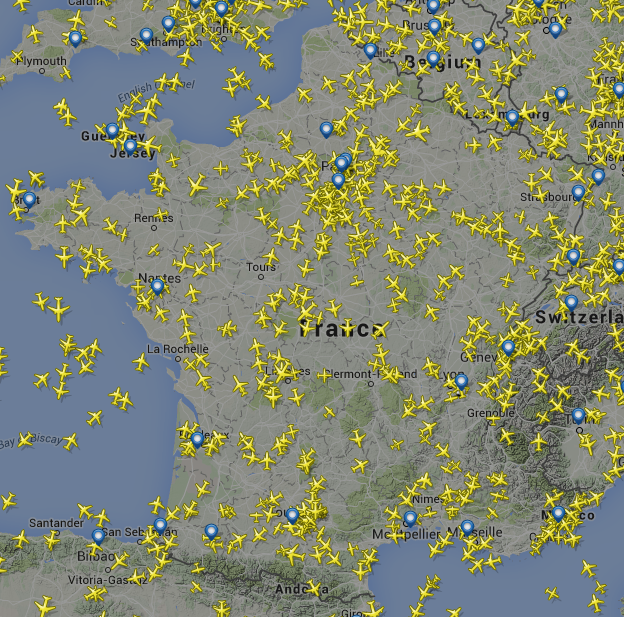
\includegraphics[width=0.5\textwidth]{Images/VolsFrance}
		\caption{Vols en temps réel}
		\label{fig:Vols}
	\end{figure}
	
	% subsection introduction (end)
	
	\subsection{Modelisation} % (fold)
	\label{sub:modelisation}
	
	Une route d'avion entre deux aéroports est effectué avec un plan de vol qui est divisé en points de passage (waypoints) à intervalle régulier (20 min). Le pilote doit suivre donc la trajectoire entre deux points de passage à chaque fois. Comme le vol est soumis au vent on doit considerer une modélisation aléatoire du processus.
	
	Dans la bibliographie la trajectoire est bien modelisé avec un process stochastique continu en temps qui est ajouté à les equations du vol (\cite{prandini2005probabilistic}). Dans cet projet on utilise la methode précedente.
	
	Plus précisement on considère des trajectoires planes, le mouvement étant décrit par 
		\begin{align}
			\mathrm d X_t &= v ~ \mathrm d t+\sigma_t ~ \mathrm d W_t
		\end{align}
ou $X_t$ répresent la position, $v$ la vitesse, $\sigma_t$ la variance et $W_t$ est un mouvement Brownian en deux dimentions. La trajectoire en chaque instant on la considère dans un repère local cntré, cet à dire la position est décomposé comme $X_t=(X_{a,t},X_{c,t})$ où $X_{a,t}$ est la composante along-track et $X_{c,t}$ est l'across-track. Donc l'équation de mouvement est:
		\begin{align}
			\mathrm d X_{a,t} &= v ~ \mathrm d t+\sigma_{a,t} ~ \mathrm d W_{a,t} \\
			\mathrm d X_{c,t} &= \sigma_{c,t} ~ \mathrm d W_{c,t}
		\end{align}
Dans ce modèle pour des raisons de pilotage on considere que quand le temps augmente on a plus de certitude sur la composante cross track mais moins sur la along-track.
\begin{align}
	X_{a,t} &\sim \mathcal{N}(vt,(r_a t)^2) \\
	X_{c,t} &\sim \mathcal{N}(0,\min(\sigma_c, (r_c t)^2))
\end{align}
	$r_a=0.25~ \mathrm{nmi min^{-1}}$ et $r_c=1/57~ \mathrm{nmi min^{-1}}$ sont facteurs fixes du modèle. Si on fait l'approximation 
	$$\min(\sigma_c, (r_c t)^2) \approx \sigma_c^2 (1-e^{-2\frac{r_c}{\sigma_c}vt}) $$
	On peut calculer $\sigma_{a,t}=r_a\sqrt{2t}$ et $\sigma_{c,t}=e^{-\frac{r_c}{\sigma_c}vt}\sqrt{2\sigma_c r_c v}$ avec Itô. On aussi une autre modelisation avec la matrice vriance/covariance pour ($t<s$):
	\begin{align}
		\mathbb{C}\mathrm{ov}(X_{a,t},X_{a,s}) &= r_a^2 t^2 \\
		\mathbb{C}\mathrm{ov}(X_{c,t},X_{c,s}) &= \sigma_{c}^2 (1-e^{-2\frac{r_c}{\sigma_c}v(s-t)})e^{-\frac{r_c}{\sigma_c}v(s-t)}
	\end{align}
	Comme sugeré dans le sujet du projet. Ce modèle est connu comme processus d'Ornstein-Uhlenbeck car la composante cross-track devient deterministe (égal à zero) dans le temps.
	Finalement juste noter que si on fait une rotation de $\theta$ degrés de notre trajectoire on doit multiplier chaque composante $X_t=(X_{a,t},X_{c,t})$ de notre processus par la matrice de rotation 
	\begin{align}
	R_{\theta} &= \left( \begin{array}{cc}
		\cos(\theta) & -\sin(\theta) \\
		\sin(\theta) & \cos(\theta)
	\end{array} \right)
	\end{align}
	chaque composante étant gaussienne avec une transformation linéaire reste gaussienne avec une moyenne de $\left( \begin{array}{c}
		vt \cos(\theta) \\ vt \sin(\theta)
	\end{array} \right)$ 
	et une matrice de covariance $R_\theta V(t) R^t(\theta)$. 
	% \TODO: Mettre la formule exacte de la covariance ?
	
	% subsection modelisation (end)
	
	\subsection{Simulation} % (fold)
	\label{sub:simulation}
	
	On considère une simulation de deux avions dans un même plan, on simule les trajectoires décrites en \ref{sub:modelisation} sur un horizon de temps de 20 minutes à une vitesse de 500 kt (926 km/h). On simule d'abord des trajectoires en parallèle et après des trajectoires qui se croissent. Les trajectoires sont discrètises uniformement avec 100 points sûr chaque trajectoire. On gardera les notations suivantes : 
	\begin{itemize}
		\item $d$ : dimention de discrétisation
		\item $\Sigma_a \in \mathbb{R}^{d \times d}$ : matrice de variance/covariance along-track
		\item $\Sigma_c \in \mathbb{R}^{d \times d}$ : matrice de variance/covariance cross-track 
	\end{itemize}
	on a donc :
	\begin{align}
		\left( \begin{array}{c}
			X^{(1)}_a \\
			X^{(1)}_c
		\end{array} \right) &\sim \mathcal{N} \left( \left[\begin{array}{c}
			vT \\ 0
		\end{array} \right] ,\left[ \begin{array}{cc}
			\Sigma_a & 0 \\
			0 & \Sigma_c
		\end{array} \right] \right)
	\end{align}
	où $X^{(1)}_a\in \mathbb{R}^d, X^{(1)}_c \in \mathbb{R}^d$ et $T=[0,\ldots,20]\in \mathbb{R}^d$ est le vecteur temps discrétisé. Si nous faisons une rotation de $\theta$ degrés, le vecteur reste gaussien avec moyenne et covariance : 
	\begin{align}
		R_{\theta} \left( \begin{array}{c}
			X^{(1)}_a \\
			X^{(1)}_c
		\end{array} \right) &\sim \mathcal{N} \left( \left[\begin{array}{c}
			\cos(\theta)vT \\ \sin(\theta)vT
		\end{array} \right] ,\left[ 
		\begin{array}{cc}
			\Sigma_a \cos^2(\theta) + \Sigma_c \sin^2(\theta)  & \sin(\theta)\cos(\theta)(\Sigma_a-\Sigma_c) \\
			\sin(\theta)\cos(\theta)(\Sigma_a-\Sigma_c) & \Sigma_a \cos^2(\theta) + \Sigma_c \sin^2(\theta)
		\end{array} 
		\right] \right)
	\end{align}
	Nous sommes intéresés en estimer la probabilité de collision c'est à dire, la probabilité de que la distance entre les avions soit inferieure à un seuil prédefini $\epsilon$.
	\begin{subequations}
	\begin{align}
		\mathbb{P}\left(\exists i~|~ \lVert X^{(1)}_{i} - X^{(2)}_{i} \rVert_2 \leq \epsilon \right)
		&= \mathbb{P}\left(\bigcup_{i=1}^{d} \lVert X^{(1)}_{i} - X^{(2)}_{i} \rVert_2 \leq \epsilon  \right)  \\
		&= \mathbb{P}\left(\min_{1\leq i\leq d} \lVert X^{(1)}_{i} - X^{(2)}_{i} \rVert_2 \leq \epsilon \right)  \\
		&= 1-\mathbb{P}\left(\forall i~|~ \lVert X^{(1)}_{i} - X^{(2)}_{i} \rVert_2 \leq \epsilon \right)
	\end{align}
	\end{subequations}
	
	% subsection simulation (end)
	
	% section presentation_du_sujet (end)
	
    \clearpage
    
    \section{Résultats}
	Les méthodes de calcul de probabilité sur des évènements rares étant vues en cours serant juste rappelés par son nom sauf pour des cas quand on fait une adaptation de la méthode.
	
	\subsection{Monte Carlo naïve} % (fold)
	\label{sub:monte_carlo_naive}
	On a fait une simulation Monte Carlo naïve pour le cas des trajectoires parallèles, une trajectoire type es montré dans la Figure \ref{fig:trajtype}. Nous avons simulé au total $10^5$ trajectoires et pour des raisons de amélioration de calcul et de simulation, nous avos decidé de simuler le processus de la difference des trajectoires $U=X^{(1)} - X^{(2)}$, dans la Figure \ref{fig:trajdiff}, on utiliserá cette figure comme référence après pour la méthode IS. Pour faire l'estimation de la probabilité de collision on utilise la fonction $\phi(U)=\mathbb{I}\left \{\min_{1\leq i \leq d} U_i \leq \epsilon \right \}$ et on calcule la probabilité de collision comme $\mathbb{E}[\phi(U)]$. L'estimation de probabilité faite avec Monte Carlo est montré dans la table \ref{tab:MC}.
	
	\begin{figure}[htbp]
		\centering
		\begin{minipage}[b]{\mylength}
			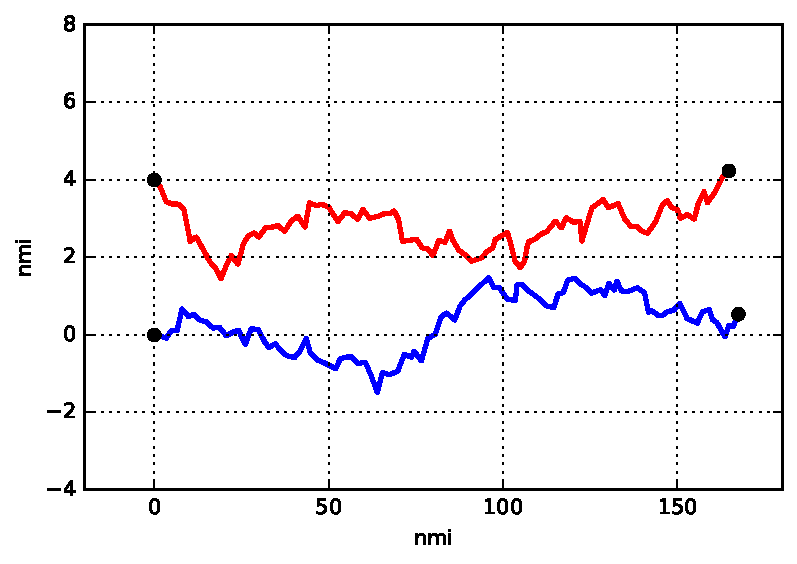
\includegraphics[width=\textwidth]{Images/Script_5_1}
			\caption{Exemple de Trajectoire}
			\label{fig:trajtype}
		\end{minipage}
		\hfill
		\begin{minipage}[b]{\mylength}
			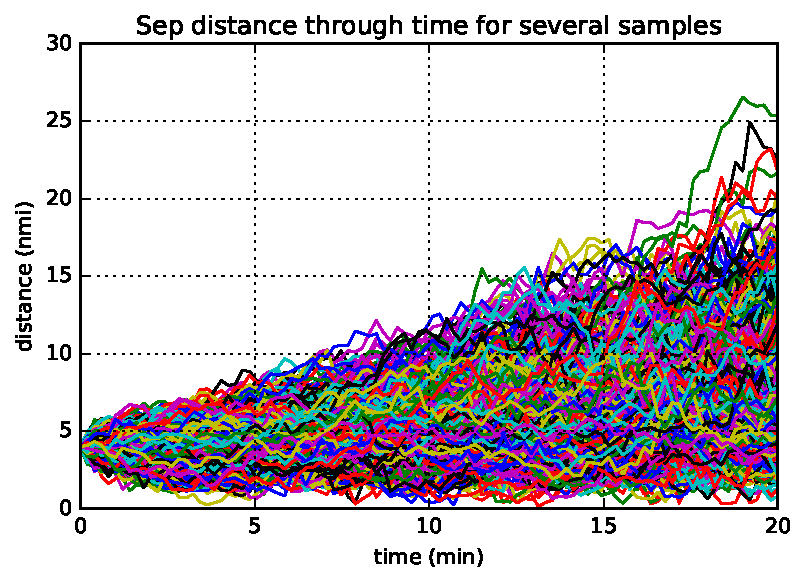
\includegraphics[width=\textwidth]{Images/Script_5_5}
			\caption{Trajectoires de $U$}
			\label{fig:trajdiff}
		\end{minipage}
	\end{figure}
	
	\begin{table}[htbp]
		\begin{center}
			\csvautobooktabular{Tables/MonteCarlo.csv}
		\end{center}
		\caption{Estimation avec Monte Carlo de la probabilité de collision}
		\label{tab:MC}
	\end{table}
	
	Dans la table \ref{tab:MC} sont representés les résultats de la méthode Monte Carlo naïve pour des distance entre 2 et 6 nmi. On a omis quelques résultats, notament quand la distance est de 6 nmi seulement avec $10^5$ simulations on pouvait arriver à des résultats non nuls. On a constaté aussi que pour $10^5$ simulations la méthode Monte Carlo marchait jusqu'à des distance de l'ordre de 6nmi. Cette méthode nous permet d'estimer des probabilités de l'ordre de $10^-5$.
	
	En analisant la table \ref{tab:MC} on constate que la méthode de Monte Cralo marche bien pour des distances petites et que après on a besoin de un nombre plus grande de simulations. Neanmoins l'erreur relatif et le nombre de simulations ne sont pas linéairement liées, c'est à dire pour ameliorer 10 fois l'erreur relatif on a besoin de plus de 10 fois le nombre de simulations utilisés anterieurement.
	
	Finalement avec les simulations Monte Carlo on a fait un histograme de la densité du minimum sur chaque trajectoire et un histograme de ça conditioné à l'évènement de collision dans les Figures \ref{fig:MChist1} et \ref{fig:MChist2}. Ces simulations sont faites à une distance de 4 nmi entre avions.
	
	\begin{figure}[htbp]
		\centering
		\begin{minipage}[b]{\mylength}
			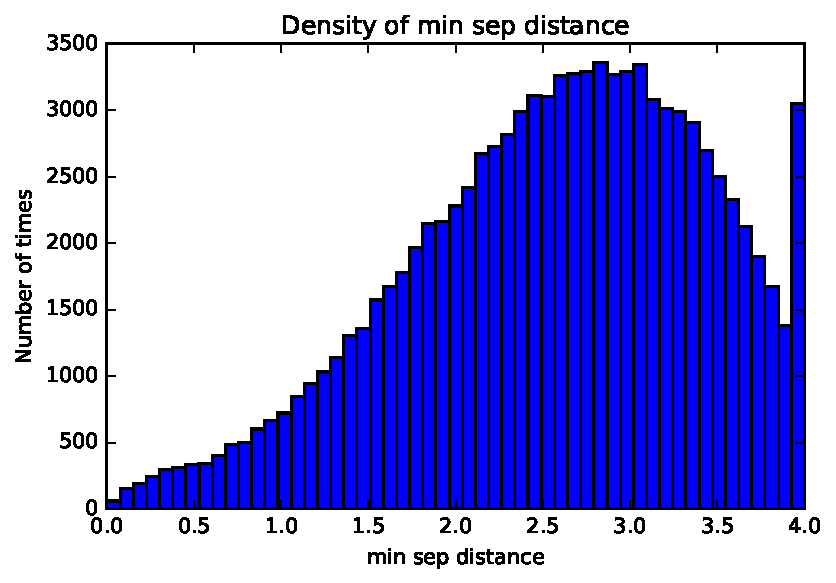
\includegraphics[width=\textwidth]{Images/Script_5_4}
			\caption{Histograme de la distance minimale}
			\label{fig:MChist1}
		\end{minipage}
		\hfill
		\begin{minipage}[b]{\mylength}
			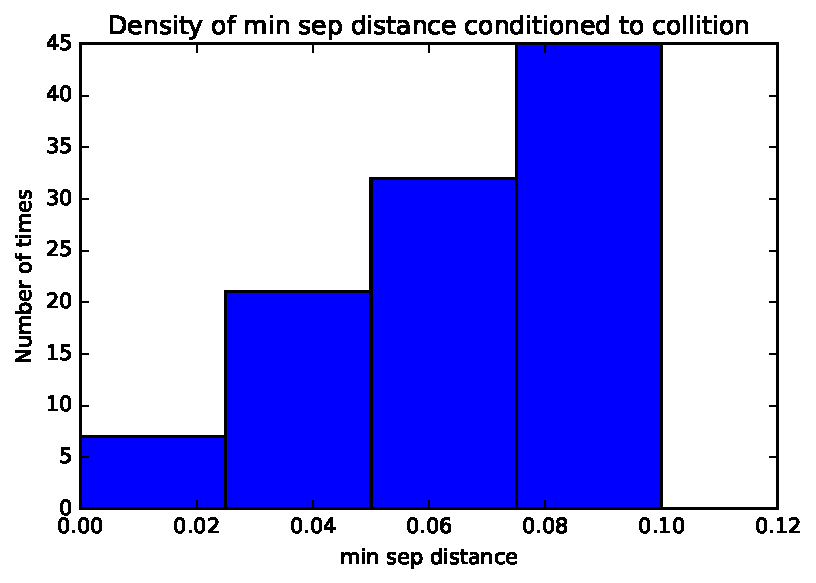
\includegraphics[width=\textwidth]{Images/Script_5_3}
			\caption{Histograme de la distance minimale conditioné à la collision}
			\label{fig:MChist2}
		\end{minipage}
	\end{figure}
	
	Dans la Figure \ref{fig:MChist1} on constate qu'il existe une grande majeurité ou le minimum se place à distance 4, celui-ci c'est le cas quand les trajectoires se eloignent l'un de l'autre au début de la simulation. On constate aussi une concentration au tour des distances entre 2 et 3.5 nmi, c'est à dire que ça c'est la distance minimale entre les deux. Finalement pour la forme de l'histogramme on pourrait dire que ça ressemble à une normale centré au tour de 2.5 et 3.0 et coupé au dela de 4, pour confirmer cette afirmation on pourrait faire un test $\chi^2$ ou  calculer la densité du minimum.Dans la Figure \ref{fig:MChist2} on constate que l'histogramme a une forme linéaire mais cependant on n'a pas suffisament d'obserbations pour confirmer cette affirmation.
	
	Dans le cas de collision on a dessiné deux histogrammes avec le temps de collision et la position de collision dans les Figures \ref{fig:MChist3} et \ref{fig:MChist4}
	
	\begin{figure}[htbp]
		\centering
		\begin{minipage}[b]{\mylength}
			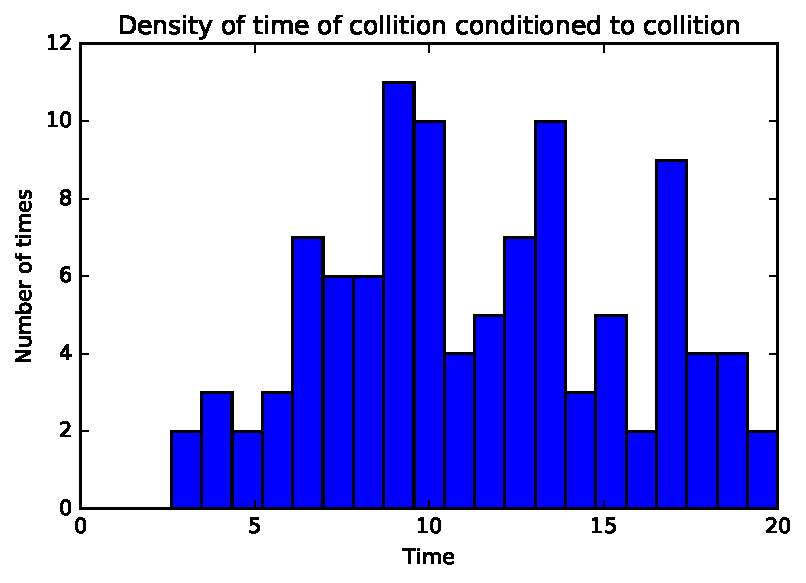
\includegraphics[width=\textwidth]{Images/Script_5_6}
			\caption{Histograme du Temps de collision entre avions}
			\label{fig:MChist3}
		\end{minipage}
		\hfill
		\begin{minipage}[b]{\mylength}
			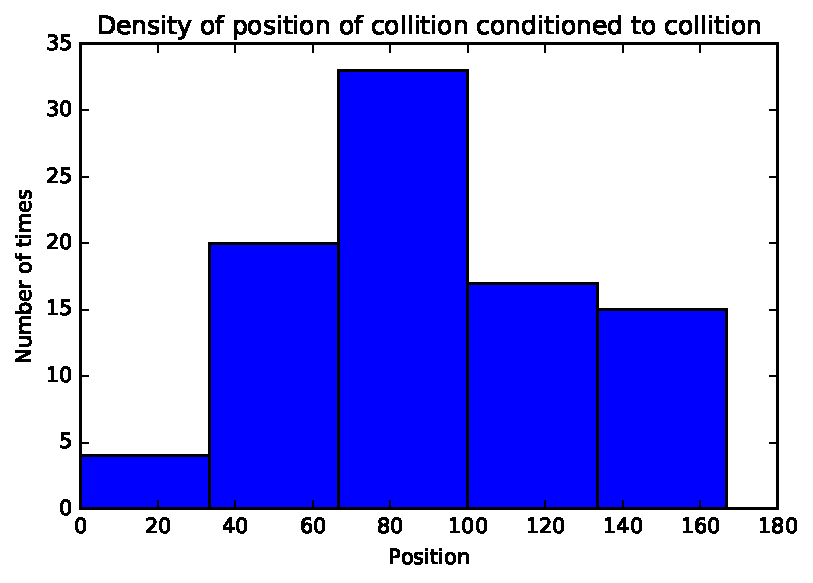
\includegraphics[width=\textwidth]{Images/Script_5_7}
			\caption{Histograme de la position de collision entre avions}
			\label{fig:MChist4}
		\end{minipage}
	\end{figure}
	
	Nous constatons que la collision tends à se produire au milieu de la trajectoire plus suivant et aussi pour la distance de collision, on constate une forme de \"toit\" dans cettes trajectoires, cette affirmation sera utilisé pour la méthode IS après.
	
	% subsection monte_carlo_naive (end)
	
	\subsection{Importance Sampling} % (fold)
	\label{sub:importance_sampling}
	
	Dans cette section on montre comment on a implementé le décentrage. Comme dans ce sujet on travail avec des gaussiennes, l'échantillonage d'importance restait valide et avec une formule assez simple comme on a vu en cours. Neanmoins le vecteur gaussienn multidimintionel $X\in \mathbb{R}^{2d}$ n'est pas centré et ça matrice de variance/covariance n'est pas l'identité. Pour résoudre cet problème on a fait deux solutions équivalents : 
	\begin{itemize}
		\item Faire un decentrage adapté au processus
		\item Normalicer le vecteur $X$ et appliquer la méthode du cours
	\end{itemize}
	Pour la première méthode on a pris à la base l'idée du decentrage:
	\begin{align}
		\mathbb{E}(f(X)) = \int f(x)p(x)~\mathrm{d}x &= \int f(x)\dfrac{p(x)}{q(x)}q(x)~\mathrm{d}x \nonumber \\
		&= \mathbb{E}_{\mathbb{Q}}(f(X)\dfrac{p(x)}{q(x)})
	\end{align}
	où $\mathbb{Q}$ es ta nouvelle distribution. On appelle aussi $L(x)=\frac{p(x)}{q(x)}$ le ratio de vraisemblances. Pour une gaussienne multidimentionelle $X \sim \mathcal{N}(\boldsymbol\mu, \Sigma)$ on a :
	\begin{align}
		p(\boldsymbol x) =
		\frac{1}{\sqrt{(2\pi)^{k}|\Sigma|}}
		\exp\left \{ -\frac{1}{2}({\mathbf x}-{\boldsymbol\mu})^\mathrm{T}{\Sigma}^{-1}({\mathbf x}-{\boldsymbol\mu})
		\right \}
	\end{align}
	Donc pour un décentrage de $\overset{\sim}{\boldsymbol X}=\boldsymbol X+ \boldsymbol \theta$ le ratio de vraisemblance est donc 
	\begin{align}
		L(\boldsymbol x) = \exp\left \{
		\boldsymbol\theta^\mathrm{T}{\Sigma}^{-1}({\mathbf x}-{\boldsymbol\mu})
		-\frac{1}{2}\boldsymbol\theta^\mathrm{T}{\Sigma}^{-1}\boldsymbol\theta
		\right \}
	\end{align}
	
	On rappelle que pour une Gaussienne standar le ratio vraisemblance est:
	\begin{align}
		L(\boldsymbol x) = \exp\left \{
		\boldsymbol\theta^\mathrm{T} {\mathbf x}
		-\frac{1}{2} \boldsymbol\theta^\mathrm{T} \boldsymbol\theta
		\right \}
	\end{align}
	Pour la deuxième méthode la procedure pour normaliser une gaussienne $X \sim \mathcal{N}(\boldsymbol 0, \Sigma)$ c'est de la centrer justa avec une modification de la probabilité qu'on cherche trouver et deuxièmement trouver sa racine carré car si on a $CC^{\mathrm{T}}=\Sigma$ alors pour une gausienne stardard $G$ on a : $CG \sim \mathcal{N} (\boldsymbol 0, C C^{\mathrm{T}})$ donc on peut simuler la variable aléatoire $X$ avec $CG$ et la formule :
	\begin{align}
		\mathbb{E}(f(X)) = \mathbb{E}(f(CG)) = 
		\mathbb{E}(
		f(C(G+{\boldsymbol \theta}))
		e^{{\boldsymbol \theta}.G
		 -\frac{1}{2} \boldsymbol\theta^\mathrm{T} \boldsymbol\theta})
	\end{align}
	Finalement pour la simulation il nous reste à regler le paramètre $\boldsymbol \theta \in \mathbb{R}^{d}$, cet paramètre est très important pour une bonne estimation pouvant amener à des grands erreur en cas d'être mal choisi. On a adopté trois méthodes pour le choix de $\boldsymbol \theta$ : un décalege constante, linéaire et toit. On a choisi ces trois décalages car le première était le plus simple à faire mais pas le meilleur, l'est autre pour des raisons de collision d'après les Figures Figure~\ref{fig:trajtype} et Figure~\ref{fig:MChist3} on voit que la collision se produit pas au début de la trajectoire mais au milieu ou à la fin. Finalement ces trois méthodes sont implementés adaptativement, c'est à dire pour chaque type de décalage on fait differents tailles de décalage. Par exemple on fait des décalages du type toit avec une variation de l'auteur du toit entre 0 et la distance entre avions.
	
	Les performances de la méthode Monte Carlo, Importance Sampling sont montrés dans la Figure~\ref{fig:ISmc} avec l'erreur dans la Figure~\ref{fig:ISmcErr}
	
	\begin{figure}[htbp]
		\centering
		\begin{minipage}[b]{\mylength}
			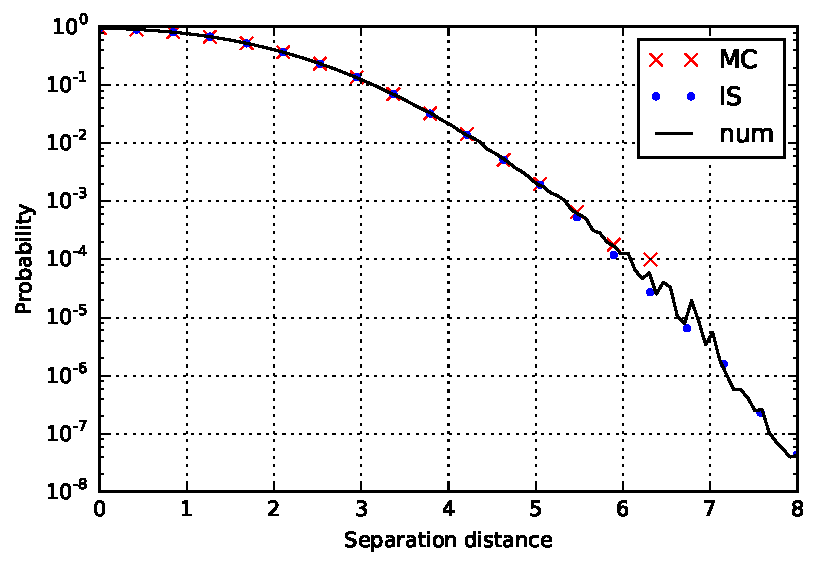
\includegraphics[width=\textwidth]{Images/Script_8_ISmc_1}
			\caption{Probabilité estimé}
			\label{fig:ISmc}
		\end{minipage}
		\hfill
		\begin{minipage}[b]{\mylength}
			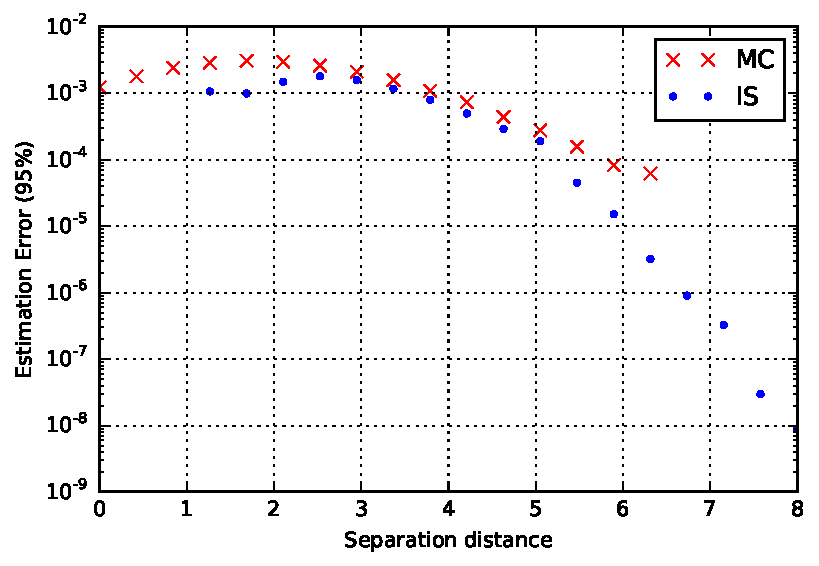
\includegraphics[width=\textwidth]{Images/Script_8_ISmc_2}
			\caption{Erreur de les méthodes}
			\label{fig:ISmcErr}
		\end{minipage}
	\end{figure}
	
	Les probabilités estimés sont montrés dans les Tables~\ref{tab:ISconst}~\ref{tab:ISlin} et \ref{tab:IStoit}
	
	\begin{table}[htbp]
		\begin{center}
			\csvautobooktabular{Tables/ISconst.csv}
		\end{center}
		\caption{Estimation avec IS type constant de la probabilité de collision}
		\label{tab:ISconst}
	\end{table}
	
	\begin{table}[htbp]
		\begin{center}
			\csvautobooktabular{Tables/ISlin.csv}
		\end{center}
		\caption{Estimation avec IS type linear de la probabilité de collision}
		\label{tab:ISlin}
	\end{table}
	
	\begin{table}[htbp]
		\begin{center}
			\csvautobooktabular{Tables/IStoit.csv}
		\end{center}
		\caption{Estimation avec IS type toit de la probabilité de collision}
		\label{tab:IStoit}
	\end{table}
	
	Dans la Table~\ref{tab:ISconst} on voit que ce n'est pas une bonne choix pour $\boldsymbol \theta$ car l'erreur relatif reste grand même quand on augmente le nombre de simulations. Par contre les estimations dans les Tables~\ref{tab:ISlin} et \ref{tab:IStoit} on obtient des bonnes approximations pour la probabilité de collision avec un erreur relatif qui reste petit. On constate aussi que quand la probabilité à estimer devient plus petite, les erreurs relatives sont plus grands.
	
	Dans les Tables on a aussi afiché le décalage $\mu$ choisi adaptativement, dans les tables on a afiché un de plusieurs runs de la méthode, on constate que la choix de $\mu$ varie et dépends de chaque simulation, mais cependant qu'elle est au tour de moins la distance entre avions et donc si on voulait une méthode robuste pour calculer la probabilité on choisirait $\mu=-\mathrm{dist}$ car elle est souvent choisie et donne des erreurs raisonables.
	%TODO: verifier "runs" et dist
	Avec la méthode obtenue par IS on a fait un histograme de la densité de probabilité, c'est à dire, on calculait pour chaque $\epsilon \in [0,4]$ la probabilité de collision ce qui nous donne la fonction de répartition et après on fait une dérivé discretisé pour obtenir la densite de probabilité. Les graphes sont afichés dans les Figures~\ref{fig:Dens1} et \ref{fig:Dens2}
	
	\begin{figure}[htbp]
		\centering
		\begin{minipage}[b]{\mylength}
			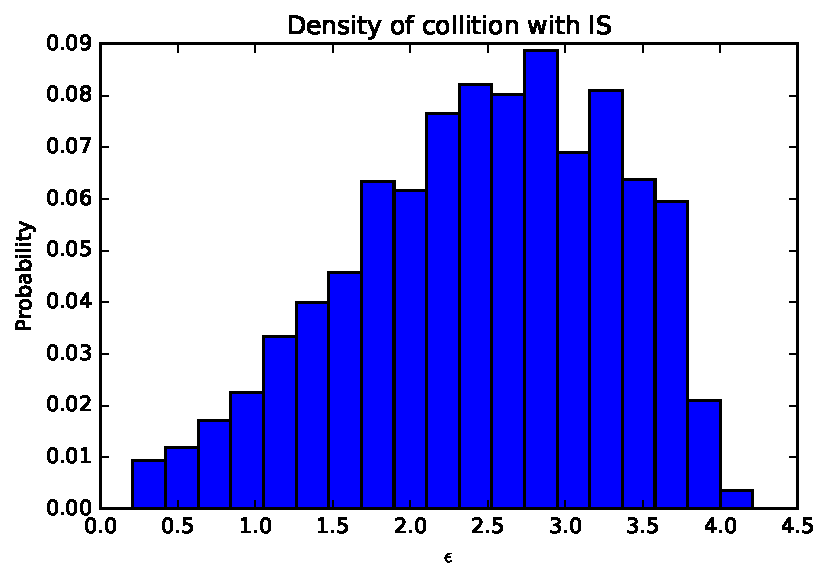
\includegraphics[width=\textwidth]{Images/Script_14_2}
			\caption{Densité de probabilité obtenue avec IS}
			\label{fig:Dens1}
		\end{minipage}
		\hfill
		\begin{minipage}[b]{\mylength}
			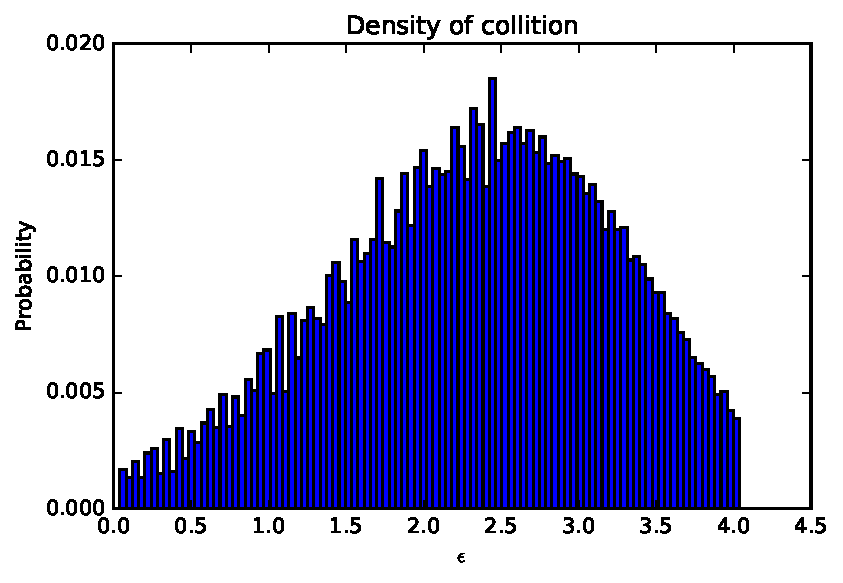
\includegraphics[width=\textwidth]{Images/Script_14_1}
			\caption{Densité de probabilité obtenue numériquement}
			\label{fig:Dens2}
		\end{minipage}
	\end{figure}
	
	Ces deux Figures sont faites pour une simulation à distance 4. La Figure~\ref{fig:Dens1} est faite avec $10^5$ simulations pour chaque $\epsilon \in [0,4]$ avec une division de 20 points, pour des raisons de vitesse. et la Figure~\ref{fig:Dens2} est faite avec 100 points. On constate une concordance entre le méthode numérique et la méthode IS.
	
	% subsection importance_sampling (end)
	
	\subsection{Méthode de Splitting} % (fold)
	\label{sub:methode_de_splitting}
	Dans cette section on implemente la méthode de splitting pour le calcul de %TODO: completar aqui
	
	On montre dans la Figure~\ref{fig:Splitting} la méthode de Splitting et le calcul par Monte Carlo de la probabilité de collision
	\begin{figure}[htbp]
		\centering
		\begin{minipage}[b]{\mylength}
			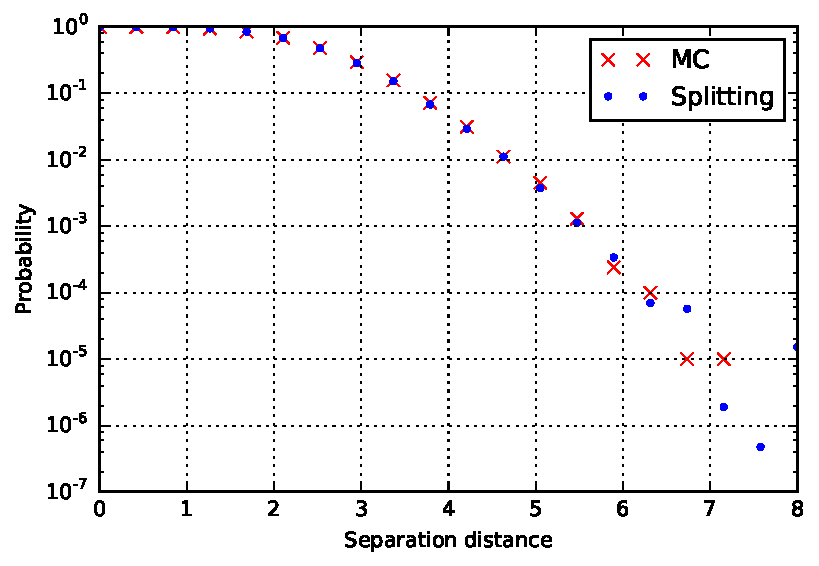
\includegraphics[width=\textwidth]{Images/Script_10_SplittingvsMC}
			\caption{Probabilité estimé avec Splitting}
			\label{fig:Splitting}
		\end{minipage}
	\end{figure}
	
	% subsection methode_de_splitting (end)
    
    \clearpage

    \section{Conclusion}


    \begin{center}
        \color{bleu303}

        \rule{0.3\textwidth}{0.2mm}\vspace*{-3.5mm}

        \rule{0.5\textwidth}{0.6mm}\vspace*{-3.8mm}

        \rule{0.3\textwidth}{0.2mm}\vspace*{-1mm}

        \sffamily FIN
    \end{center}
    
     \clearpage
        \section{Références bibliographiques}
        {
        \renewcommand{\section}[2]{} % pour virer le titre "Références"
        \nocite{*}
        \bibliographystyle{alpha}
        \bibliography{rapport_Modal_SNA}
        }

    
\end{document}
